\section{Opgave 1 - MeeMoo state machine}
\begin{enumerate}
	\item[1)]
	
	Som anmodet i opgavebeskrivelsen, har vi skrevet programmet som en Moore state machine først. Altså, ændrer Moore output værdi, alt efter hvilken state den skiftes til. Denne værdi er clock-reguleret.
	
	Derefter har vi tilføjet Mealy state machinen inde i state-init, hvor den regulerer Mealy output værdien efter værdierne for A og B. Denne værdi er IKKE clock-reguleret.
	VHDL-koden for programmet er følgende:
	
\begin{lstlisting}[caption={Kode for MeeMoo state machine},label={lst:MeeMooSM}]
library ieee;
use ieee.std_logic_1164.all;

entity MeeMooSM is
	port (clk, reset, a, b : in std_logic;
	moo_out, mee_out : out std_logic);
end MeeMooSM;

architecture three_processes of MeeMooSM is
	type state is (state_idle, state_init, state_active);
	signal present_state, next_state : state;
	
	begin

		state_reg: process (clk, reset)
		begin
			if reset = '0' then
				present_state <= state_idle;
			elsif rising_edge(clk) then
				present_state <= next_state;
			end if;
		end process;

		outputs: process (present_state, a, b)
		begin	
			case present_state is
			when state_idle => 
				moo_out <= '0';
				mee_out <= '0';
			when state_init => 
				moo_out <= '1';
				if a = '0' and b = '1' then
					mee_out <= '0';
				elsif a = '1' and b = '1' then
					mee_out <= '1';
				end if;
			when others => 
				moo_out <= '1';
				mee_out <= '0';
			end case;
		end process;

		nxt_state: process (present_state, a, b)
		begin
			case present_state is
			when state_idle =>
				if a = '0' then
					next_state <= state_idle;
				elsif a = '1' then
					next_state <= state_init;
				end if;
			when state_init =>
				if b = '0' and a = '0' then
					next_state <= state_idle;
				elsif b = '1' and a = '0' then
					next_state <= state_active;
				else 
					next_state <= state_init;
				end if;
			when state_active =>
				next_state <= state_idle;
			end case;
		end process;
end three_processes;


\end{lstlisting}
\item[2)]
På figur \ref{fig:meemoofuncsim} ses en functional simulation af state machinen. Det ses at den opfærer sig som forventet.
\begin{figure}[h]
	\centering
	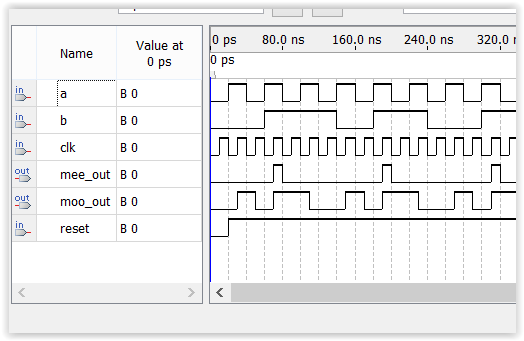
\includegraphics[scale=0.7]{pictures/Oevelse7/opg1/meemoofuncsim.JPG}
	\caption{Functional simulation af MeeMoo state machine.}
	\label{fig:meemoofuncsim}
\end{figure}

Vi downloader til vores DE2-board hvor vores moore output er på LEDR0 og mealey output er på LEDR1. Clock er på KEY0 og reset er KEY1. A er switch1 og B er switch0.
\begin{figure}[h]
	\centering
	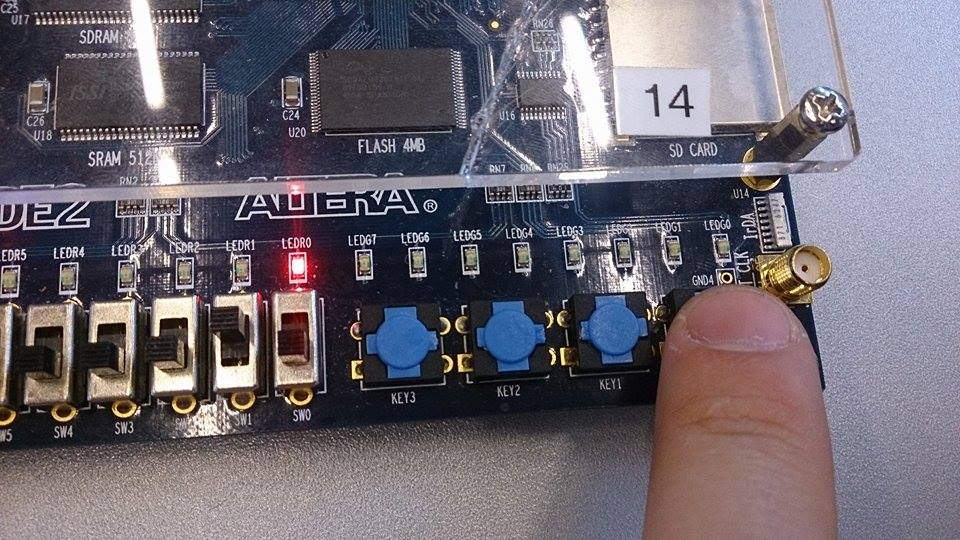
\includegraphics[scale=0.7]{pictures/Oevelse7/opg1/BA100MooMeeINIT.JPG}
	\caption{MeeMoo er i init-state og AB er 10/0}
	\label{fig:BA100MooMeeINIT}
\end{figure}
		
\begin{figure}[h]
	\centering
	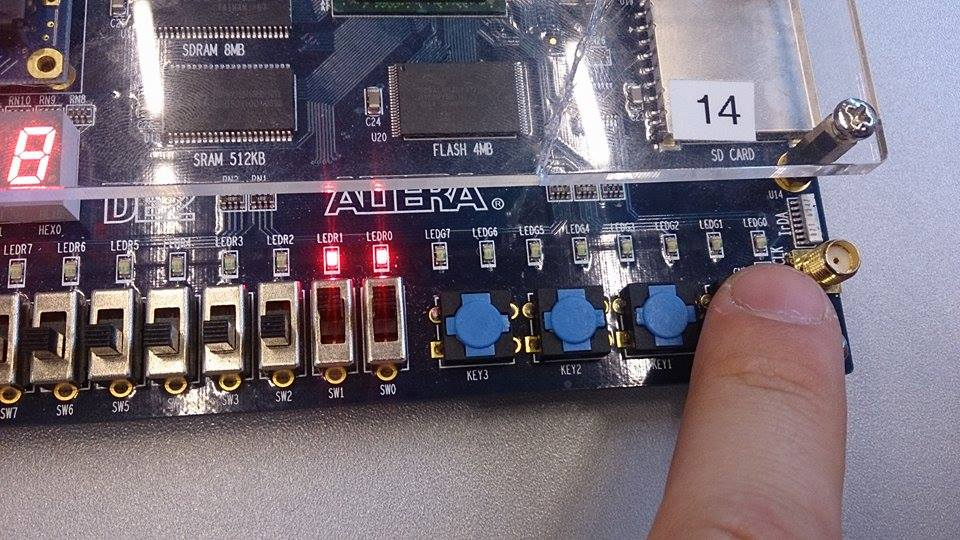
\includegraphics[scale=0.75]{pictures/Oevelse7/opg1/BA111MooMeeINIT.JPG}
	\caption{MeeMoo er i init-state og AB er 11/1}
	\label{fig:BA111MooMeeINIT}
\end{figure}


\begin{figure}[h]
	\centering
	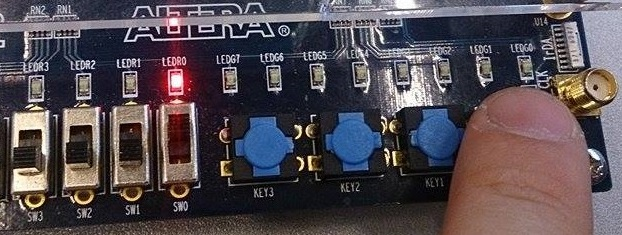
\includegraphics[scale=0.8]{pictures/Oevelse7/opg1/BA010MooMeeACTIVE.JPG}
	\caption{MeeMoo er i active-state og AB er 01/0}
	\label{fig:BA010MooMeeACTIVE}
\end{figure}

\end{enumerate}
	\newpage